\documentclass[11pt,a4j,fleqn]{jarticle}
\usepackage{amsmath,amsthm,amssymb}
\usepackage[dvipdfmx]{graphicx}

\title{課題2 包絡線定理}
\author{花嶋 陽}
\date{2014/6/7}


\begin{document}

\maketitle

\section{はじめに}
包絡線定理は、経済学において効用最大化や費用最小化等の最大化、最小化問題を解く際に活用されます。
以下では、単純な関数で包絡線定理について説明した後、包絡線を描画するプログラムのコードについて解説します。



\section{包絡線定理}

関数
\[
f(x, t) = t x - t^2
\]
が与えられているとします。tをパラメータと見て、x−y平面上の直線
\[
l_t:y = t x - t^2
\]
を考えると、tの値を変化させるごとに1本の直線が引けます。
tの値をいろいろ変えて直線l_tをいくつも描いたものが図1、図2です。
図を見ると、直線l_tの通過領域はある曲線(Cと呼ぶことにします)の下側全体となっていることが分かります。
この曲線を表す関数をF(x)とおくと、

\[
F(x) = \max_tf(x, t)                                
\]

となります。ここでfをtについて平方完成すると
\[
f(x, t) = -\left(t - \frac{x}{2}\right)^2 + \frac{x^2}{4}
\]
となるので、fはt = x/2で最大値x^2/4となることがわかります。よって、

\[
F(x) = \frac{x^2}{4}
\]

となります。
次に、図より曲線Cと各l_tとが必ず接する形で交点を持つことが見てとれますが、これを確かめましょう。
先のtについての最大化問題の解を$t*(x)$と置きます。
各x = \bar{x}において、$F(\bar{x}) = f(t*(\bar{x}), \bar{x})$なので、x = \bar{x}で
曲線Cと直線l_{t*(\bar{x})}は交わります。
また、Cの傾きはF'(\bar{x}) = \bar{x}/2であり、直線l_{t*(\bar{x})}は

\[
y = \frac{\bar{x}}{2}x - \frac{x^2}{4}
\]

となるので、その傾きも$\bar{x}/2$であり、たしかに曲線Cと直線l_{t*(\bar{x})}は
任意のxにおいて接することが分かりました。
以上のことから、F'(x)を計算するのに、

\[
\frac{\partial f}{\partial x}(t*(x), x)
\]

を計算すればよいことがわかります。
つまり、関数f(x,t)について、
\[
F(x) = \max_tf(x, t)
\]
とし、F(x)とf(x, t)はxについて微分可能だとします。
ここで、各xに対して最大値を与えるtをt*(x)と表します。このとき、
\[
F(x) = \frac{\partial f}{\partial x}(t*(x), x)
\]
が成り立ちます。これを包絡線定理と言います。


\begin{figure}
 \centering
 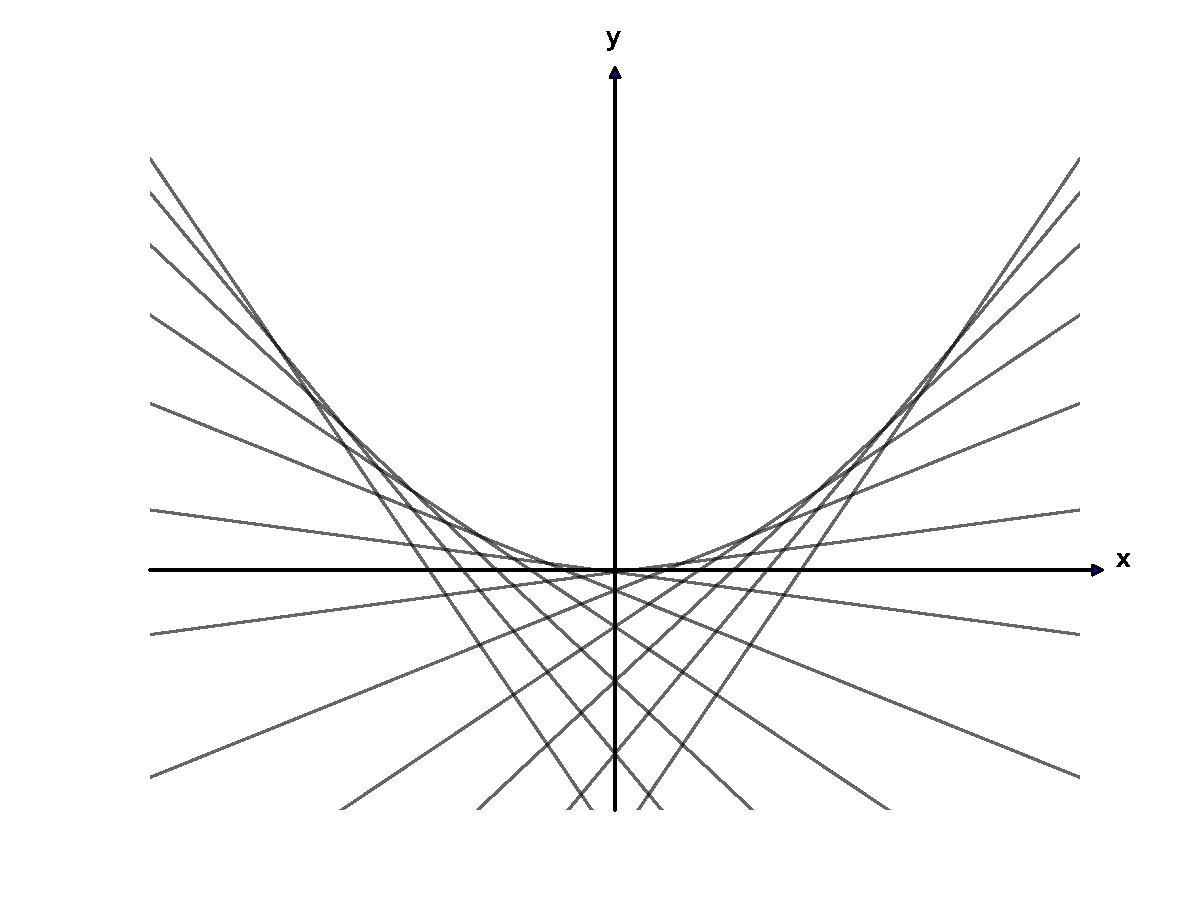
\includegraphics[scale=0.25]{envelope0.pdf}
 \caption{接線の本数少なめ}
 \label{fig:1}
\end{figure}

\begin{figure}
 \centering
 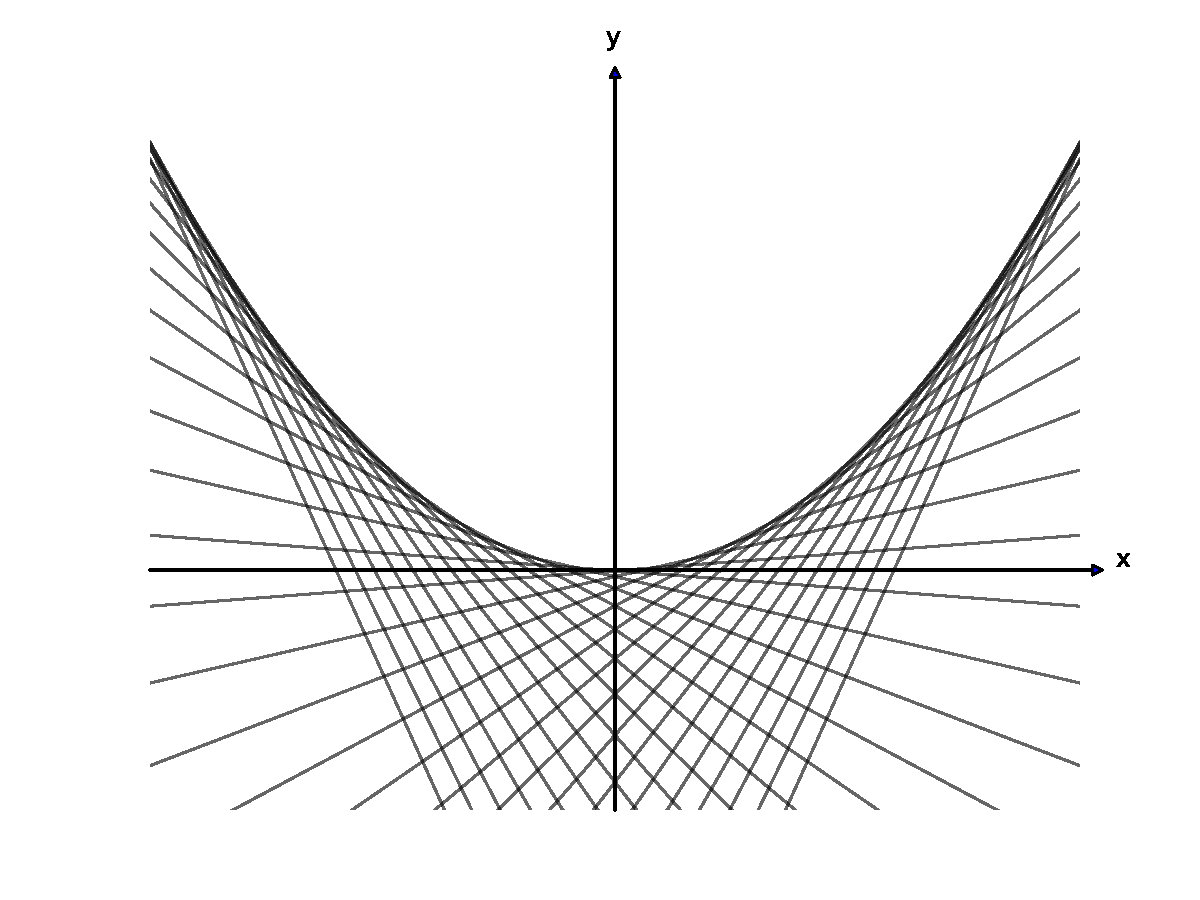
\includegraphics[scale=0.25]{envelope1.pdf}
 \caption{接線の本数多め}
 \label{fig:2}
\end{figure}



\section{Pythonプログラム}

\begin{quote}
\begin{verbatim}
# -*- coding: utf-8 -*-

import matplotlib.pyplot as plt
import numpy as np
from mpl_toolkits.axes_grid.axislines import SubplotZero


# 図の背景の諸体裁を設定

# 作図スペースを用意。	
fig = plt.figure(1)
ax = SubplotZero(fig, 111)
fig.add_subplot(ax)

# 軸の設定
ax.axhline(linewidth=1.2, color="black")
ax.axvline(linewidth=1.2, color="black")

# 軸に矢印
for direction in ["xzero", "yzero"]:
	ax.axis[direction].set_axisline_style("-|>")
	ax.axis[direction].set_visible(True)

# 四方の軸を消す。	
for direction in ["left", "right", "bottom", "top"]:
	ax.axis[direction].set_visible(False)

# 軸に名前を付ける。位置は適宜設定。	
plt.figtext(0.93, 0.37, 'x')  
plt.figtext(0.505, 0.95, 'y')

# 軸の目盛を消す。表示するy軸の範囲を設定(グラフが見易くなるよう適宜設定)。
plt.xticks([])
plt.yticks([])		
plt.ylim(-3.5,6.5)


# 図を描く条件設定

# 元になる関数を定義
def f(x, t):
    return t * x - t**2

# 変数
savever = 'png' # 'png' or 'pdf'
fignum = 0 # 0 or 1

if fignum == 0:  
    p = 5    #xの範囲 -p<=x<=p (左右対称にするため)
    r = 2    #tの範囲 -r<=t<=r (同上)
    n = 12   #接線の本数

if fignum == 1:
    p = 5
    r = 3
    n = 30
	
# 包絡線を作る
x = np.linspace(-p,p,2)    # 直線なのでプロットする点は2点でいいかと。
t = np.linspace(-r,r,n)  # 傾きはn-1等分で均等に。lispaceで範囲内をn-1等分したarrayを用意。
for i in t:
	y = f(x, t=i)
	ax.plot(x, y, 'k-', linewidth=1.0, alpha=0.6)
plt.savefig('envelope' + str(fignum) + '.' + savever)
plt.show()

工夫した所は、tの値をlinspaceによるarrayで用意したことです。
課題としては、yの表示の範囲を変数の変更に応じて自動で調整できればと思います。

\end{verbatim}
\end{quote}


\begin{thebibliography}{0}
\bibitem{OyamaYasuda11}
尾山大輔・安田洋祐「経済学で出る包絡線定理」『経済セミナー』2011年10・11月号.
\end{thebibliography}

\end{document}